\section{Software}\label{sec:software}
Nachdem das Kapitel Hardware ausführlich behandelt wurde, muss nun noch die Software dazu beschrieben werden. Der verwendete Mikrocontroller legt die Verwendung des Software Development Kit \cite{nordic_sdk} (SDK) nahe. Dies ist eine Sammlung von Beispielen, Librarys und vorcompilierten Codes. Verwendet wurde die Version v12.3.0. Die SDK ist aufgrund des verwendeten integrierten Bluetooth-Stack wichtig. Dieser ist im sogenannten Softdevice enthalten. Um ihn nutzen zu können, verwenden wir den S132. Dieser und die nötige Initialisierungen des Bluetooth-Stacks waren in dem Beispielprojekt Uartc in der Central-Rolle vorhanden. Dadurch wurde das ganze Projekt auf diesem Beispiel aufgebaut. Der Softdevice und die SDK legen einige Abstraktions-Layer auf die Hardware. Diese sind in Abbildung \ref{fig:Software_Layers} visualisiert. Die wichtigsten Module des SDK werden im Kapitel \ref{sec:nordicsdk} erklärt, falls weitere Informationen gewünscht sind, wird auf die offizielle Dokumentation verwiesen \cite{nordic_info}. Wichtig für dieses Kapitel ist, dass der beschriebene Software-Zustand dem Soll-Zustand entspricht. Die Abweichungen sind im Kapitel Validierung genauer beschrieben.


\begin{figure}[htbp!!!!]
	\centering
	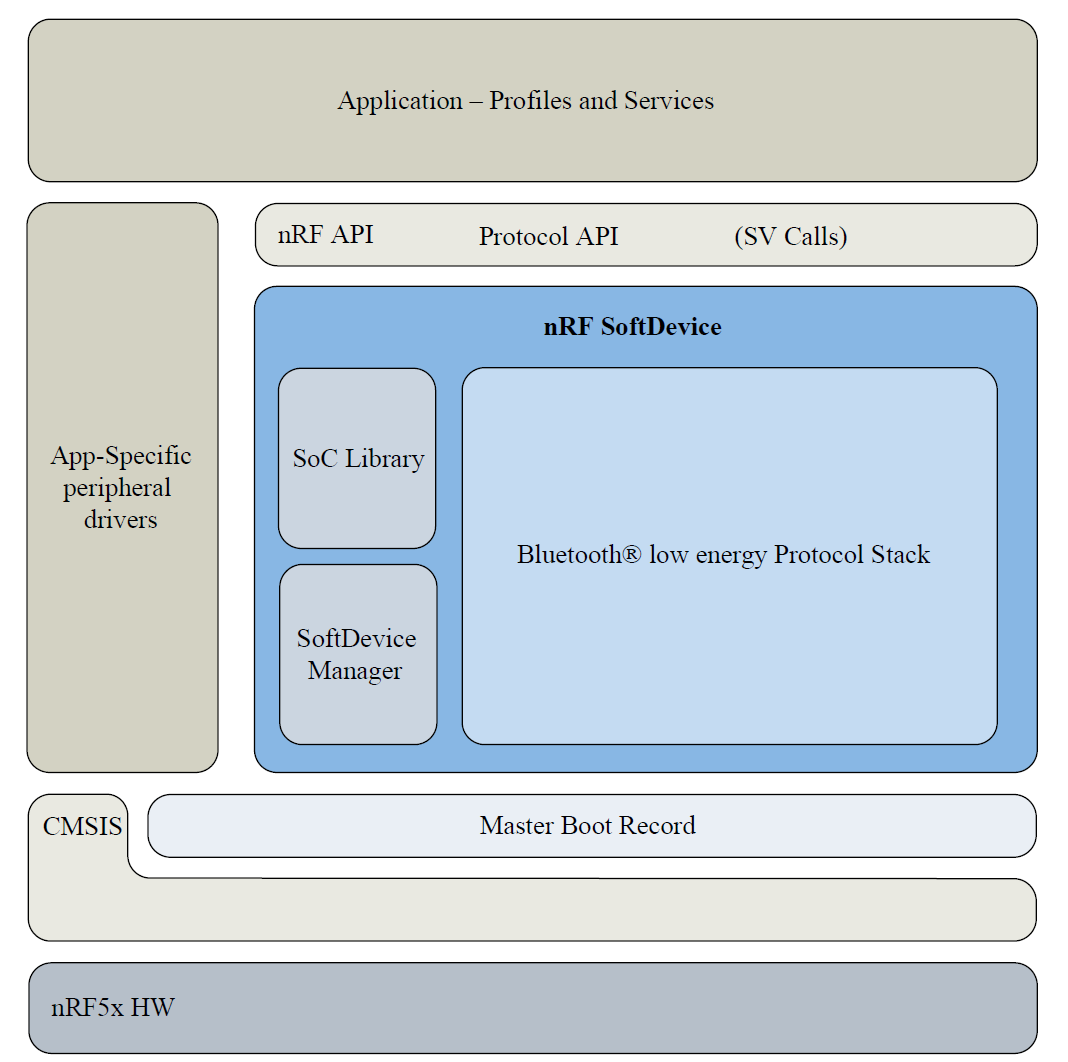
\includegraphics[width=0.9\textwidth]{Data/Software_Layers.PNG}
	\caption[Software:Layers]{Aufbau der Software auf der Hardware}
	\label{fig:Software_Layers}
\end{figure} 

Der eigentliche Programmaufbau ist eine Statemachine, welche so aufgebaut ist, dass alle Events möglichst kurz gehalten wurden. Jedoch hat dies relativ viele Flags zur Folge. Anschliessend werden die Events entsprechend ihrer Priorität verarbeitet. Die Prioritäten ergeben sich aus der Else IF im Wait State, genaueres dazu wird im Kapitel \ref{sec:stateMachine} beschrieben. Dadurch entsteht ein pollendes Programm mit Prioritäten, wie in Abbildung \ref{fig:Software_approach} dargestellt.

\begin{figure}[htbp!!!!]
	\centering
	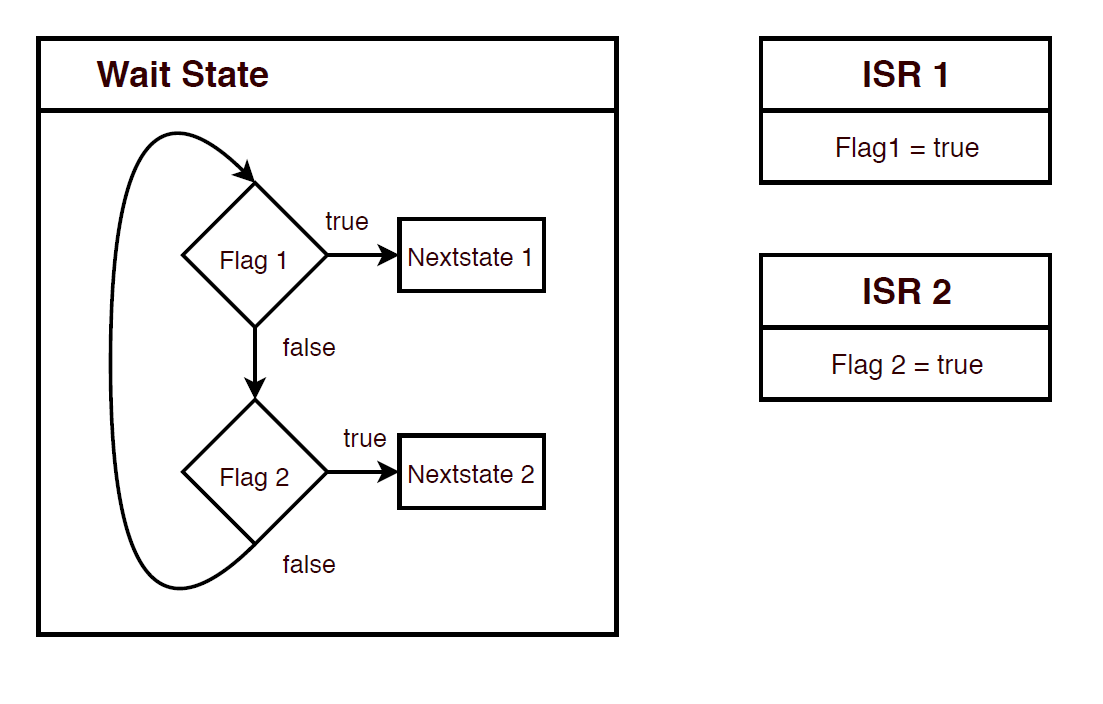
\includegraphics[width=0.8\textwidth]{Data/Software_Pollend}
	\caption[Software:Pollend]{Konzept der pollenden Software}
	\label{fig:Software_approach}
\end{figure}

Das Programm wurde in verschiedene Module unterteilt, um die Leserlichkeit zu verbessern. Die Unterteilung wurde entsprechend der Funktionen gemacht. Im Hauptmodul (Main) sind nur die Statmachine und die Interrupthandler vorhanden. Folglich wurde ein Modul für die BLE-Funktionalitäten geschrieben und eines für die SD-Karte. Ein weiters Modul existiert für die Batterie-Funktionalitäten. Dieses ist jedoch nicht implementiert und enthält nur Dummy-Funktionen.






